\documentclass[11pt,a4paper]{article}
\usepackage[utf8]{inputenc}
\usepackage[spanish]{babel}
\usepackage{amsmath}
\usepackage{amsfonts}
\usepackage{amssymb}
\usepackage{graphicx}
\usepackage{url}
\author{Ignacio Ram\'{\i}rez}
\title{Detecci\'{o}n de M\'{a}quinas de Escribir}

\begin{document}

\maketitle

\section{Descripción del problema}

Se trata de clasificar (agrupar) los documentos según tengan la misma letra.
Tener los documentos agrupados, en este caso por tipo de letra, puede ahorrar
mucho trabajo y proveer información adicional para facilitar la interpretación.

Más aún, si se llegara al caso ideal de identificar una máquina en particular, se podría relacionar los documentos producidos por esa máquina con un lugar físico puntual, ayudando a determinar más aún su procedencia.

Lo anterior se podría hacer por ejemplo si se tiene en cuenta no sólo el tipo de letra sino la intensidad de las distintas letras, los pequeños desplazamientos verticales de algunos caracteres por la propia máquina, etc.


La figura~\ref{fig:letras} muestra algunos ejemplos.

\begin{figure*}
\centering%
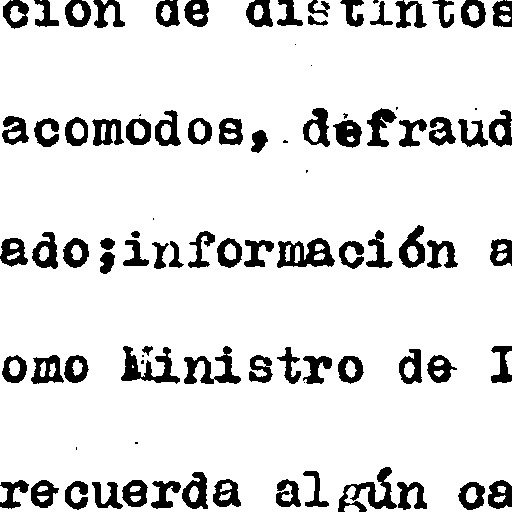
\includegraphics[width=0.2\textwidth]{r0566_0019.jpg}%
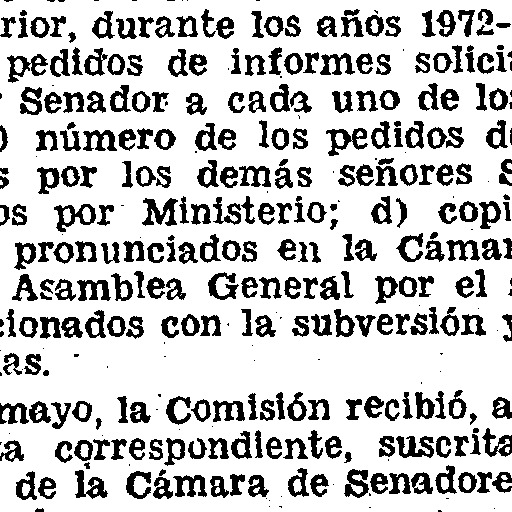
\includegraphics[width=0.2\textwidth]{r0566_0689.jpg}%
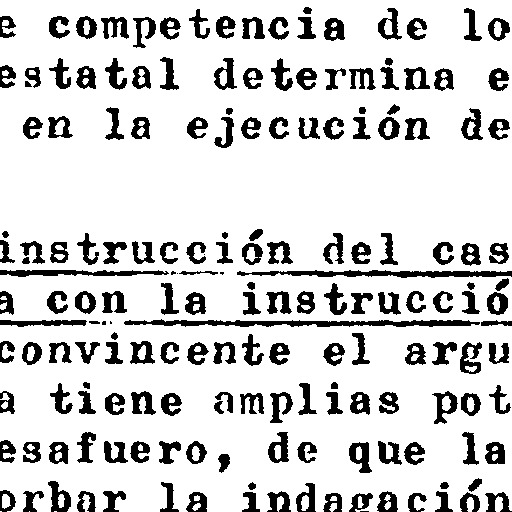
\includegraphics[width=0.2\textwidth]{r0566_0949.jpg}%
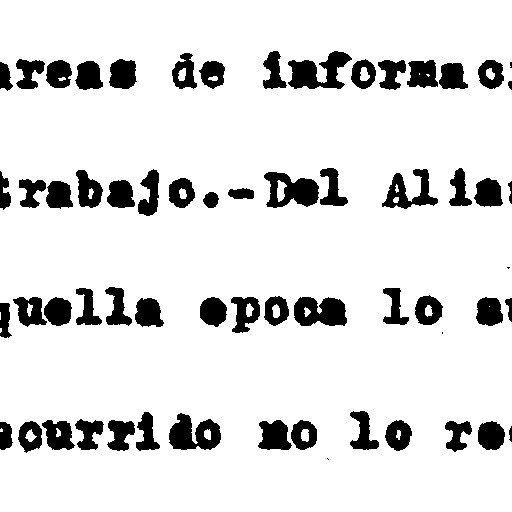
\includegraphics[width=0.2\textwidth]{r0566_0037.jpg}\\
\centering%
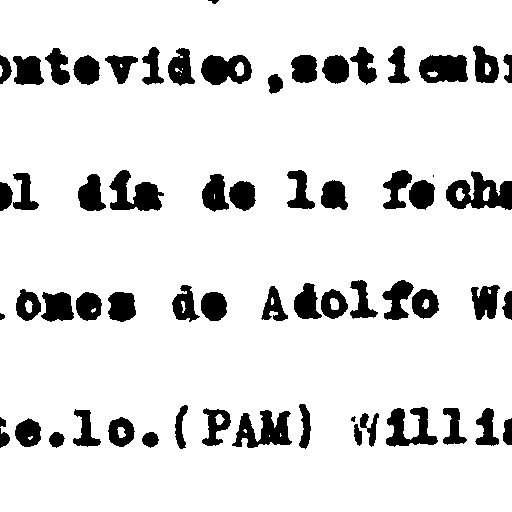
\includegraphics[width=0.2\textwidth]{r0566_0038.jpg}%
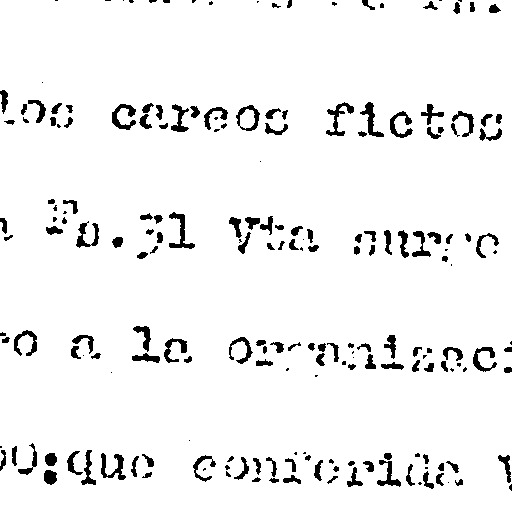
\includegraphics[width=0.2\textwidth]{r0566_0064.jpg}%
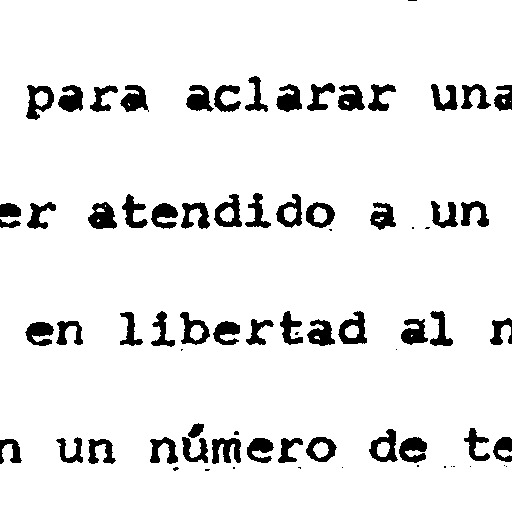
\includegraphics[width=0.2\textwidth]{r0566_0080.jpg}%
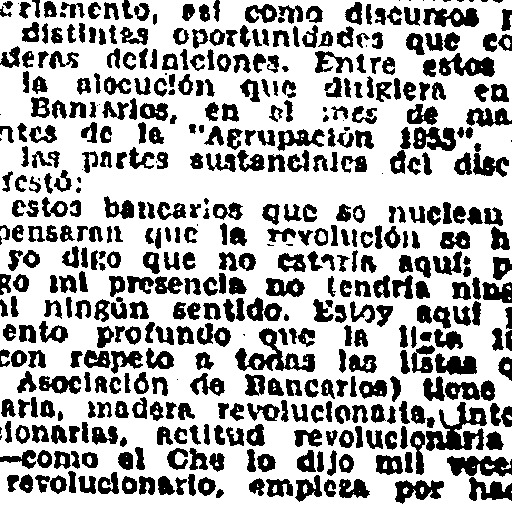
\includegraphics[width=0.2\textwidth]{r0566_0121.jpg}\\
\centering%
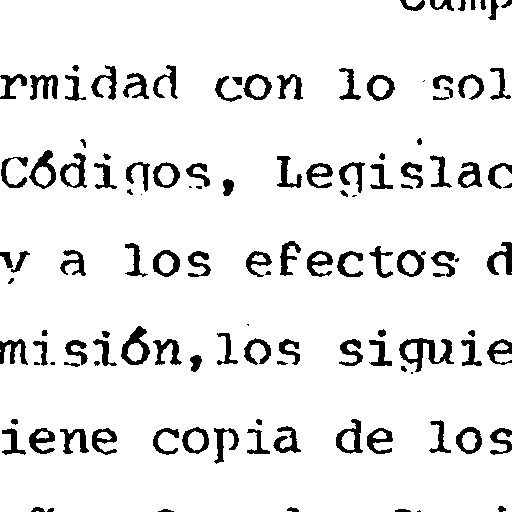
\includegraphics[width=0.2\textwidth]{r0566_0138.jpg}%
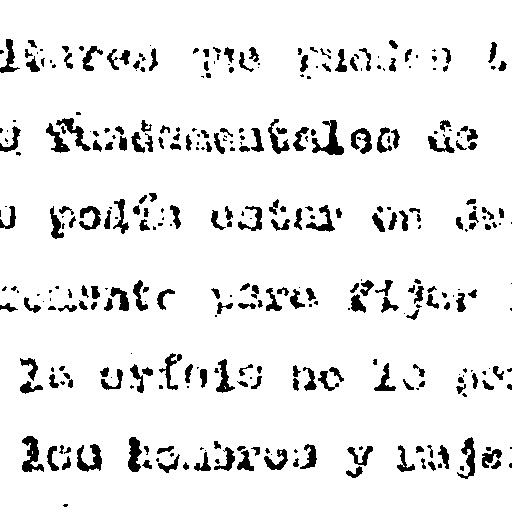
\includegraphics[width=0.2\textwidth]{r0566_0148.jpg}%
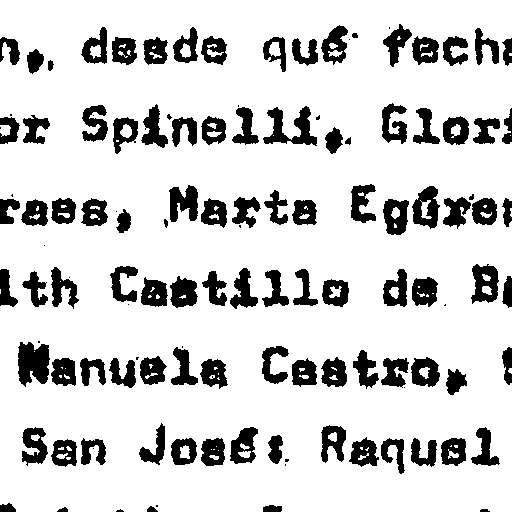
\includegraphics[width=0.2\textwidth]{r0566_0219.jpg}%
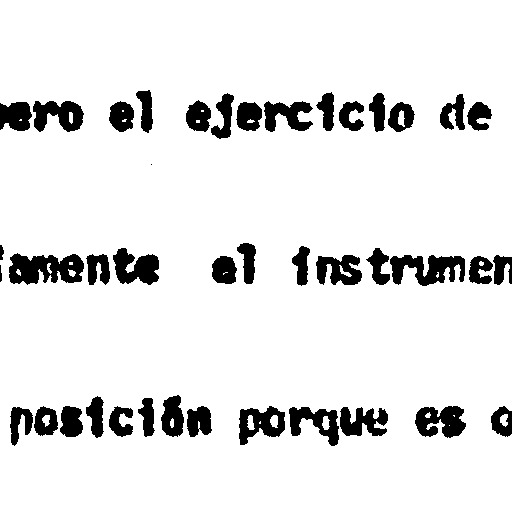
\includegraphics[width=0.2\textwidth]{r0566_0369.jpg}\\
\centering%
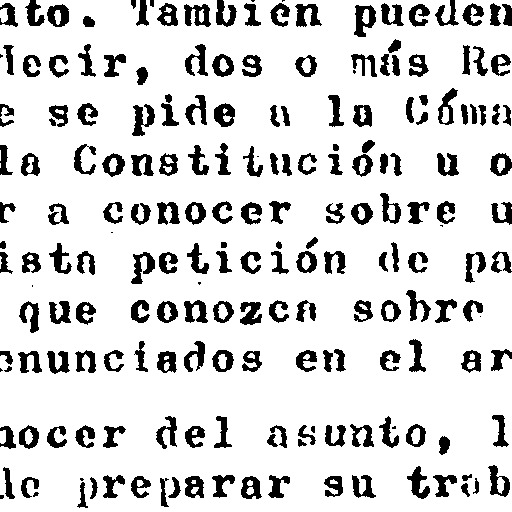
\includegraphics[width=0.2\textwidth]{r0566_0512.jpg}%
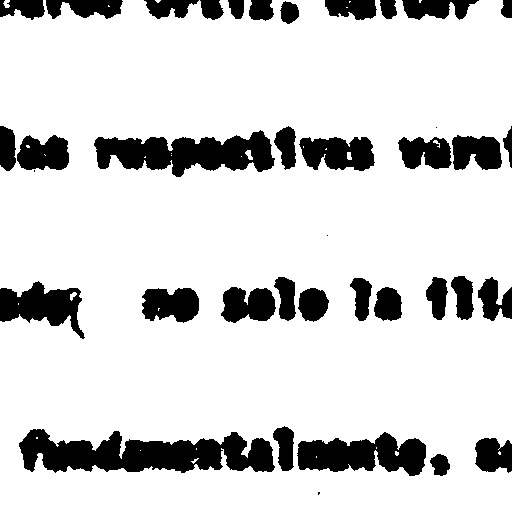
\includegraphics[width=0.2\textwidth]{r0566_0539.jpg}%
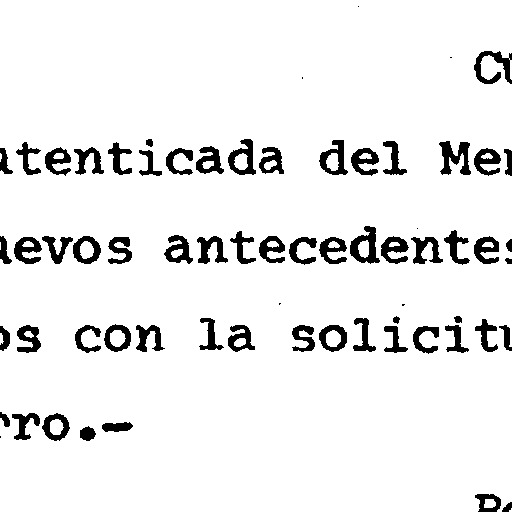
\includegraphics[width=0.2\textwidth]{r0566_0569.jpg}%
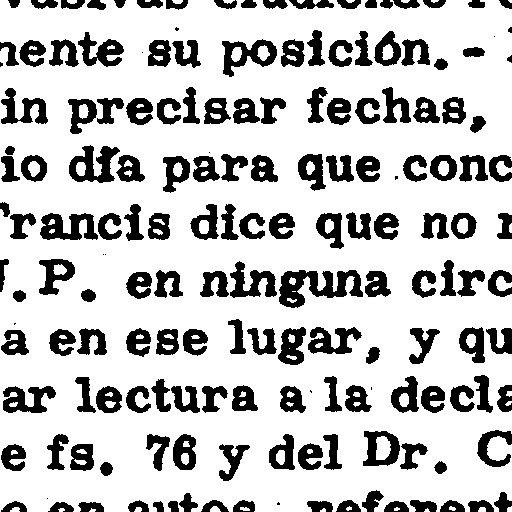
\includegraphics[width=0.2\textwidth]{r0566_0599.jpg}\\
%\centering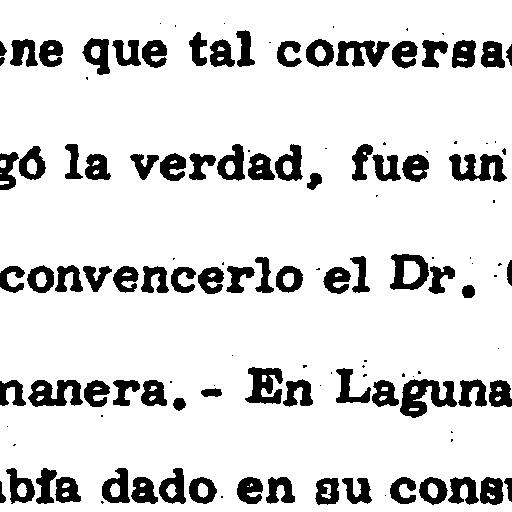
\includegraphics[width=0.24\textwidth]{r0566_0600.jpg}%
%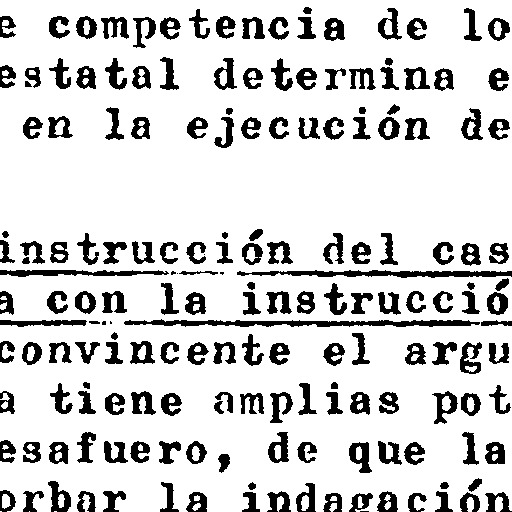
\includegraphics[width=0.24\textwidth]{r0566_0949.jpg}
\caption{\label{fig:letras}Ejemplos de distintos tipos de letra.}
%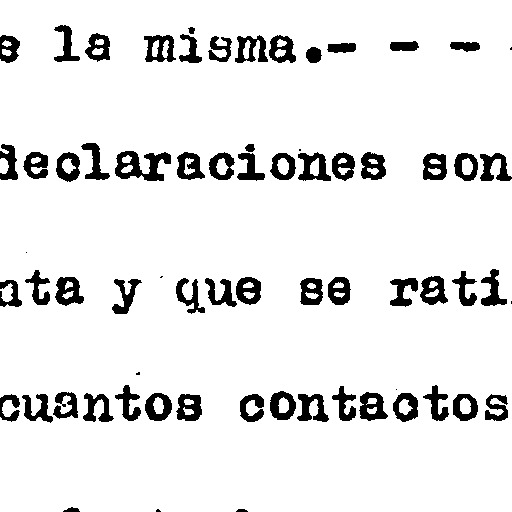
\includegraphics[width=0.24\textwidth]{r0566_0027.jpg}%
%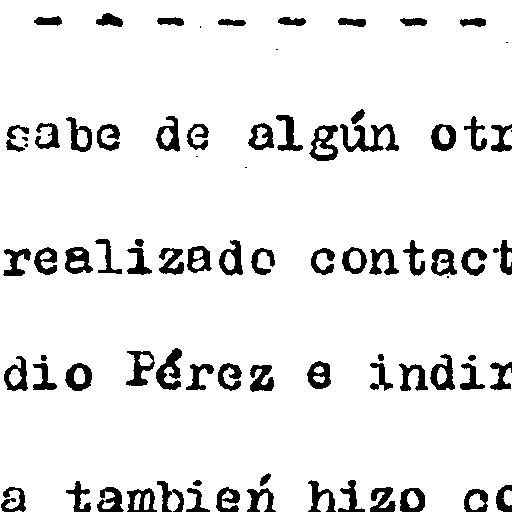
\includegraphics[width=0.24\textwidth]{r0566_0028.jpg}%
\end{figure*}

\section{Consideraciones técnicas}

Este es un problema abierto. Tengo varias ideas sobre cómo tratarlo, pero son demasiado difíciles para resumir ahora (en una versión posterior intentaré proponer algunas técnicas). Como problema abierto, se recomienda utilizar Python para su desarrollo y así aprovechar la facilidad de generación de gráficas y la enorme cantidad de bibliotecas que dispone (numpy, scipy).


\end{document}